\section{Reinforcement Learning Framework}\raggedbottom 
The main components of the reinforcement learning framework are the \textit{agent} and the \textit{environment}.

An agent interacts with the \textit{environment} over time, by taking in the environment state, which is usually denoted as $s$ or $x$. Within this work, we will always use $s$ for the state.
The agent evaluates the state and decides on an \textit{action} (denoted as $a$), based on the current state. 

A  problem distinct to reinforcement learning is the one of exploration and exploitation. In order to learn the best behaviour the \textit{agent} needs to make sure to explore the \textit{environment}. Insufficient exploration can lead to suboptimal policies.

Whenever the agent interact with the environment, a\textit{reward} and the next state are given to him in return.
Depending on whether the environment is terminal or not, an additional value denoting if the environment has terminated is received. 
The Atari games considered within this work all terminate eather if the player has lost or won the game.

\begin{figure}
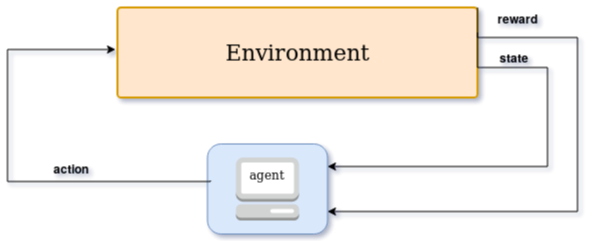
\includegraphics[width=90mm]{bilder/RLFramework.png}
\caption{Agent interacting with the environment}
\end{figure}


\subsection{Elements of Reinforcement Learning}
\citet{Sut98} names 4 other core elements of the reinforcement learning framework.

\textbf{Policy}

The behaviour of the agent at any given time $t$ is determined by the \textit{policy}. A policy $\pi$ can roughly be described as a mapping of states to an action or a distribution over actions. 
We denote the probability of an action $a$ being taken at state $s$ at time $t$ under a policy $\pi$ as
\begin{equation}
P_\pi( a \mid s_t) = \pi(a \mid s_t)  
\end{equation}
Within this work, the policy is always stochastic and the probability distribution over actions is denoted as $\pi (\bullet \mid s)$
\pagebreak

\textbf{Reward Signal}

The problem posed by an environment is defined through the reward function. 

The goal of the learning agent is to receive the maximum accumulated future reward at any given time. One of the most important features of reinfocement learning is the fact, that rewards are often very delayed. 

Connecting the delayed reward with the actions that caused it is a key task of reinforcement learning.
Good examples are games like Pong or Breakout, where the reward is caused by successfully playing a ball, but only received many frames later.

Games like chess pose an even bigger problem, since every move can play an important role in winning the game. Good opening moves can strongly impact if the game is lost or won 100 moves later.

The reward received by an agent at timestep $t$ will be denoted as $r_t$.

\textbf{Value Function}

The value of a state represents the sum of the future rewards, and indicate the long term desirability of states.

The value of a state at timestep $t$ under a policy $\pi$ is given through the expectancy of the \textit{return} $R_t$ , which is the possible accumulated future reward denoted as $V(s)$ and given by:

\begin{equation}
{
V^\pi (s) = E_\pi \{R_t \mid s_t = s\} = E_\pi \left\{ \sum_{k=0}^\infty \gamma^k r_{t+k+1} \mid s_t = s \right\}
}
\end{equation}

In accordance with this, we define the state-action value $Q(s,a)$, which is simply the expected return, if the action $a$ is taken at state $s$.

\begin{equation}
{
Q^\pi (s,a) = E_\pi \{R_t \mid s_t = s, a_t = a\} = E_\pi \left\{ \sum_{k=0}^\infty \gamma^k r_{t+k+1} \mid s_t = s, a_t = a \right\}
}
\end{equation}

This is a good place to additionally define the advantage $A^\pi(s,a)$ of  $s$ given $a$ is taken.

\begin{equation}
A^\pi(s,a) = Q^\pi(s,a)-V^\pi(s,a)
\label{adv}
\end{equation}

The advantage of an action given a state denotes, how much better this action is, compared to the average action.

\textbf{Environment Model}

In order to solve a problem, a model of the environment can be learned and used for planning. A model can be used to predict future states and rewards before they happen.
Model-based and model-free reinforcement learning methods, which explicitly learn by trial and error both play an important role in reinforcement learning.

Within this thesis we will only look at model-free methods. Rather than learning a model, the agent learns directly through trajectories sampled from the environment.

\pagebreak

\subsection{Markov Decision Process} 

We can describe the sequential decision making process of the \textit{agent} more formally as a Markov decision process (MDP).

The sequential decision making process is given by a sequence of states, actions and rewards:

$s_0, a_0, r_0, s_1, a_1, r_1, s_2, a_2, r_2, \dots, s_t,a_t,r_t, s_{t+1}$

We will refer to such sequences as \textit{trajectories}

Within this thesis, we assume the environment to be finite.

We call a state \textit{Markov} or say it has \textit{Markov property} if it only depends on it's predecessor rather than the whole history.
\begin{equation}
P(s_{t+1} = s', r_{t+1} = r' \mid s_t, a_t, r_t, s_{t-1}, \dots ,r_1,a_0,s_0) = P(s_{t+1} = s', r_{t+1} = r' \mid s_t,a_t)
\end{equation}

A finite discounted Markov decision process $MDP(S,A,P_a,R_a,\gamma)$ contains a finite set of states $S$, 
a finite set of actions $A$,
the transition probablity to end up in state $s'$ if action $a$ is taken in state $s$ : 
\begin{equation}
P^a_{s s'} = Pr(s_{t+1} = s' \mid s_t = s, a_t = a)
\end{equation}

the reward function $R^a_{s s'}$,
and the discount factor $\gamma  \in [0,1)$, used to define the importance of immediate reward in contrast to future reward. 

\subsection{Deep Reinforcement Learning}
In contrast to directly mapping an input to an output value, deep learning algorithms contain so called \textit{hidden layers}.


Usually a transformation or activation function is applied to the input if each hidden layer. Rectified linear units (ReLU), the tanh or the sigmoid function can be named as popular activaton functions.
After feeding an input into the network and calculation an error value, the weights are adjusted through backpropagation.

Convolutional neural networks (CNN) were inspired by visual neuroscience and are great tools to process image data. CNNs mainly consist of convolutional layers, pooling layers and fully connected layers.
Other relevant approaches are recurrent neural networks (RNN) or long short term memory networks (LSTM). Both mimic functions of a memory and have started to play bigger roles within the field of deep reinforcement learning recently.

Combining deep learning methods with reinforcement learning methods was a major breakthrough, enabeling reinforcement learning methods to be successfully applied to complex problems like those posed by the Atari 2600 console. \citep{deeprlLi}

Within this thesis, we will work with CNNs, consisting of convolutional layers, dense layers and ReLU activation functions.

We use convolutional layers to extract features from image data. By moving a filters over the image, and calculating the weighted sum of the filter and the respective parts of the images the output is calculated. 

The outputs are weighted sums of parts from the original image.
The \textit{stride} denotes how much a filter is shifted before being applied to the image again. Multiple filters can be are used, to receive many different features.

\begin{figure}
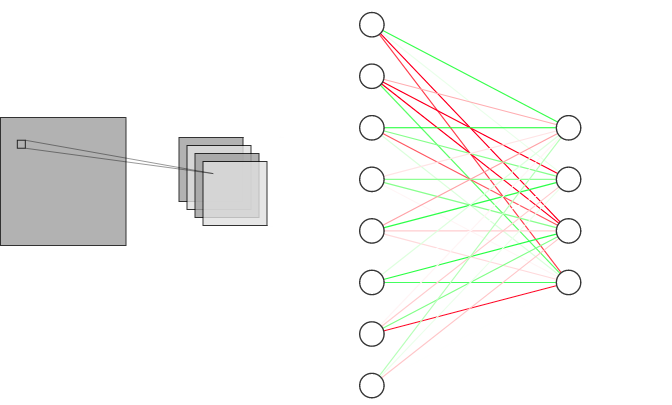
\includegraphics[scale=0.5]{bilder/deeplayers.png}
\caption{A convolutional (left) and fully connected (right) layer.
}
\label{networks}
\end{figure}

Fully Connected Layers are used to weight the input  and map it to the output space. 

Each 'Neuron' or element in the output layer, holds a weighted sum of every input element. (\ref{networks})

The ReLU function simply changes all negative values to 0, while positive values remain untouched:

\begin{equation}
ReLU (x) = 
\begin{cases}
x & \text{if x >0} \\
0 & else
\end{cases}
\end{equation}


\pagebreak